\section{Services}

\subsection{Test Services}

We can separate services into test and operational services.
Table \ref{tab:testservers} lists known test services supporting
ECH. All of those below .ie and my-own.net were setup by the 
DEfO project.

\small
\begin{longtblr} [
        caption = {Test Services with ECH},
        label = {tab:testservers}
    ] {
        colspec = {| l | p{0.7\linewidth} |},
        rowhead = 1
    }
    \hline
        Name & Details\\
    \hline
        defo.ie & \url{https://defo.ie/ech-check.php} is often used to check ECH\\
        & ECH keys are rotated hourly, private usable for 3 hours, ECHConfigList in DNS contains only latest public\\
    \hline
        draft-13.esni.defo.ie & different server technology instances on different ports as listed at \url{https://defo.ie/}, e.g., \url{https://draft-13.esni.defo.ie:10413} is served by nginx\\
        & ECH keys are rotated hourly, private usable for 3 hours, ECHConfigList in DNS contains only latest public\\
    \hline
        test.defo.ie & hosts a number of ECH server setups with good and variously bad configurations - see
        \url{https://test.defo.ie/iframes_tests} describes those and allows a browser to attempt connections to
        each via Iframes\\
        & ECH keys/configs are static for these setups\\
    \hline
        foo.ie & \url{https://foo.ie/ech-check.php} was setup used to check the defo.ie setup was easily replicated\\
        & ECH keys are rotated hourly, private usable for 3 hours, ECHConfigList in DNS contains only latest public\\
    \hline
        my-own.net & this was test the impact of having the same ECH keys on
        port 443 (\url{https://my-own.net/ech-check.php}) and another port  
        (\url{https://my-own.net:8443/ech-check.php})  - at one point that made a difference to browsers\\
        & ECH keys are rotated hourly, private usable for 3 hours, ECHConfigList in DNS contains only latest public\\
    \hline
        tls-ech.dev & \url{https://tls-ech.dev/} was setup by the boringssl developers as a test server that uses
        boringssl\\ 
        & \todo{Check ECH key rotation}\\
    \hline
        Cloudflare & \url{https://cloudflare-ech.com/cdn-cgi/trace} is a test page
           setup by cloudflare that reports on ECH success/failure\\
        & apparently, the server implementation and infrastucrure are part of Cloudflare's normal setup\\
        & a similar test service used to be available at \url{https://crypto.cloudflare.com/cdn-cgi/trace} but
        that was turned off around the time that ECH was re-enabled for Cloudflare customers\\
        & ECH keys are rotated hourly, private usable for N hours, ECHConfigList in DNS contains only latest public\\
        & \todo{Check what N for private key usability}\\

    \hline
        rfc5746.mywaifu.best & this ECH-enabled web page (\url{https://rfc5746.mywaifu.best/}) seems to have been setup 
        as an ECH test site by someone using DEfO artefacts (nginx and documentation) but without any contact
        having happened between the person who set that up and any of the DEfO-project participants\\
        & the person who set this up documented some of that at \url{https://ckcr4lyf.github.io/tech-notes/services/nginx/nginx-ech.html}\\

    \hline
\end{longtblr}
\normalsize

\subsection{Operational Services}

The only operational ECH service we know of is Cloudflare's deployment.
However, that is non-negligible.  Cloudflare earlier enabled ECH but disabled
it soon after in
October 2023~\footnote{\url{https://community.cloudflare.com/t/early-hints-and-encrypted-client-hello-ech-are-currently-disabled-globally/567730}}
as it caused some back-end issues. They then re-enabled ECH in October 2024.
Our understanding of Cloudflare's deployment is that ECH is enabled by 
default for their "free" tier customers, but that paying customers have to
take action to enable ECH.

In contrast, non-paying customers are not provided with a control to disable
only ECH - they have to downgrade to TLSv1.2 in order to disable ECH. This
is something that has been seen in recent weeks after the Russian government
started blocking use of ECH to
Cloudflare.~\footnote{\url{https://betanews.com/2024/11/20/encrypted-client-hello-didnt-solve-censorship-but-still-may-have-a-role-to-play/}}

\subsection{Domain Probe Data}

As part of our DEfO test setup, we have a web page where you can enter a DNS
name and port and a script on our server will check if ECH is enabled for a web
server at the name and port. (That's at
\url{https://test.defo.ie/domainechprobe.php}.) Data is only stored if there is
an HTTPS resource record for the name and port, if there is not we store
nothing. In cases where this is an HTTPS resource record, we only store the
name and port, whether the HTTPS value includes an "ech=" field, if there is,
whether or not ECH worked using our ECH-enabled curl as the client. We also
store the HTTPS resource record value, unless there are CNAMES or other
kinds of re-direction involved.

We can use this data to get some further insight into services for which ECH
is enabled. For now, we are not publishing the raw data - while data for the most
recent 50 queries is shown on the web page, if we wanted to publish the raw
data, we'd have to enable some form of consent for users, and it's not clear
that'd be a) easy or b) worthwhile.

Figure \ref{fig:qtimes} shows the (small) numbers of queries made since August
2024. We can see a noticeable uptick in accesses just-before and after Russia
block Cloudflare's ECH service. We also see some usage (at least 15 cases) that
appear to indicate Russian web site owners may be using this service to check
whether or not they have successfully disable ECH. (The pattern is two quick
accesses to the same name/port, the first of which indicates ECH worked, and
the second that the HTTPS RR no longer contains an "ech=" value.)

\begin{figure}
	\centering
	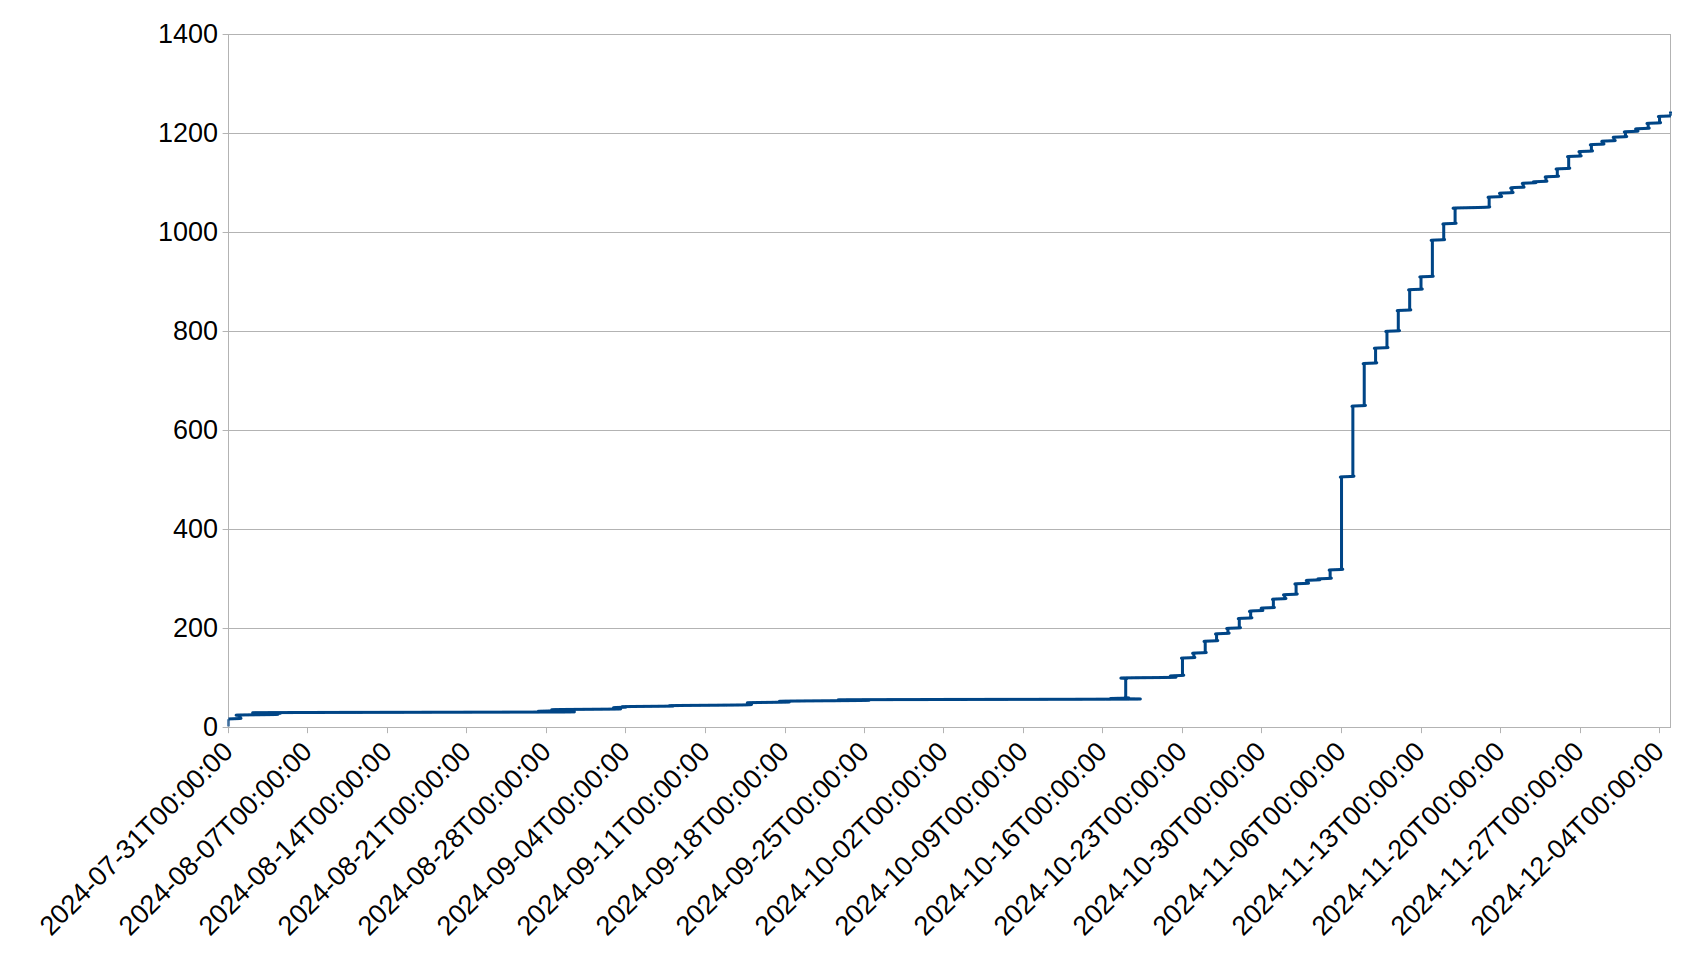
\includegraphics[width=0.8\textwidth,keepaspectratio]{domainprobequeries.png}
		\caption[clustediag]{Cumulative number of queries seen at 
        \url{https://test.defo.ie/domainechprobe.php} versus time. 
        The total number of queries is 1244.} 
	\label{fig:qtimes}
\end{figure}

The 1244 queries involved 517 unique domain names (117 of which are under
the ".ru" ccTLD). The most commonly queried name is "youtube.com" (131 times),
for which ECH is not currently enabled. Some 354 names were only queried 
once, and 86 were queried twice.

